\pdfsuppresswarningpagegroup=1

\documentclass[
    %handout,
]{beamer}

\usetheme{Boadilla}
\usecolortheme{seahorse}
\usepackage{pifont}
\usepackage{pgfplots}
\usepackage{svg}
\usepackage{t1enc}
\usepackage{bbding}
\usepackage[hungarian]{babel}
\usepackage[none]{hyphenat}

\pgfplotsset{
    tick label style = {font = {\fontsize{8 pt}{14 pt}\selectfont}},
    every axis label = {font = {\fontsize{8 pt}{14 pt}\selectfont}},
    label style = {font = {\fontsize{10 pt}{20pt}\selectfont}},
    legend style = {font = {\fontsize{6 pt}{10 pt}\selectfont}},
}

\titlegraphic{
\includegraphics[width=2cm]{elte_cimer_szines}}
\title[HoloDB]{HoloDB: szintetikus adatok on-the-fly szolgáltatása relációs adatbázisként}
\author[Horváth Dávid]{Horváth Dávid \\ ~ \\ { \footnotesize Témavezető: Dr. Vincellér Zoltán, Mesteroktató }}
\institute[ELTE-IK]{ELTE Informatikai Kar, Információs Rendszerek Tanszék}
\date{2023}

\newcommand{\slidetitle}[2]{\frametitle{{\small #1 ~ \ding{226} ~ } \normalsize \textbf{#2} }}

\newcommand{\greencheck}{{ \color{green!65!black} \ding{51} }}

\begin{document}
\beamertemplatenavigationsymbolsempty

\frame{\titlepage}

\AtBeginSection[]
{
    \begin{frame}
        \frametitle{Tartalom}
        \tableofcontents[currentsection]
    \end{frame}
}

\section{Bevezetés: adatbázist akarok, most!}
\def\sectionshorttitle{Bevezetés}

\begin{frame}
    \slidetitle{\sectionshorttitle}{Adatbázist akarok, most!}
    
    \begin{itemize}
        \setlength\itemsep{1.5em}
        \item adatfüggő mockok és stubok biztosítása \pause
        \item integrációs és egyéb tesztelés \pause
        \item gyors prototípusgyártás, kísérletezés draft adatbázisokkal \pause
        \item rövid demonstrációk, prezentációk
    \end{itemize}
\end{frame}

\begin{frame}
    \slidetitle{\sectionshorttitle}{Alaptézis}
    
    \centering
    
    \includegraphics[height=0.3\textwidth]{diagram/test-with-data}
    
    \begin{minipage}[b]{0.8\textwidth}
        \justifying
        Igen gyakran ütközünk abba a problémába,
        hogy adott struktúrájú és szemantikájú,
        viszonylag rövid életű adatbázist kell biztosítani,
        a produkciós adatokra vonatkozó speciális követelmények nélkül.
    \end{minipage}
\end{frame}

\section{Körkép: a létező (kerülő)megoldások}
\def\sectionshorttitle{Körkép}

\begin{frame}
    \slidetitle{\sectionshorttitle}{Megközelítések}
    
    \begin{itemize}
        \setlength\itemsep{0.5em}
        \item produkciós adatbázis másolatának használata \pause
        \item anonimizálás \pause
        \item adatgenerálás \pause
        \item lekérdezések mockolása \pause
        \item egyéb?
    \end{itemize}
\end{frame}

\begin{frame}
    \slidetitle{\sectionshorttitle}{Nagyteljesítményű megoldások}
    
    Nagyteljesítményű megoldások
\end{frame}

\begin{frame}
    \slidetitle{\sectionshorttitle}{Egy másfajta lehetséges ihletforrás}
    
    Generált világ: milyen egyszerű egy nagy rakás adatot kapni
    de nem indexelt, és nem is ez történik
\end{frame}

\section{Egy új megoldás körvonalai: HoloDB}
\def\sectionshorttitle{HoloDB}

\begin{frame}
    \slidetitle{\sectionshorttitle}{Elvárások egy új megoldással szemben}
    
    \begin{itemize}
        \setlength\itemsep{0.5em}
        \item relációs adatmodellre épül \pause
        \item deklaratív, finomhangolható, könnyen bővíthető \pause
        \item nem szükséges forrásadatbázis, de mintaként használható \pause
        \item nincs preparálási folyamat, szinte azonnal elindul \pause
        \item óriás adatmennyiséget is képes szimulálni, szinte tárhelyigény nélkül \pause
        \item az adatokat csak elérésükkor, on-the-fly számítja \pause
        \item a runtime teljesítmény kielégítő \pause
        \item determinisztikus, konzisztens, skálázható \pause
        \item opcionálisan írható
    \end{itemize}
\end{frame}

\begin{frame}
    \slidetitle{\sectionshorttitle}{Mit tapasztal a felhasználó?}
    
    konfig;
    azonnal elindul;
    kis költséggel fut;
    úgy viselkedik, mint egy valódi adatbázis
\end{frame}

\section{A HoloDB architektúrája}
\def\sectionshorttitle{Architektúra}

\begin{frame}
    \slidetitle{\sectionshorttitle}{Vázlatos architektúraábra}
    
    Architektúraábra, storage API,
    majd a virtual impl.-ban az értékkiosztás/kétf. é.k. kiemelése
\end{frame}

\begin{frame}
    \slidetitle{\sectionshorttitle}{Segédtípusok}
    
    Fontosabb interfészek
\end{frame}

\begin{frame}
    \slidetitle{\sectionshorttitle}{LargeInteger}
    
    LargeInteger: leírás + benchmark
\end{frame}

\begin{frame}
    \slidetitle{\sectionshorttitle}{TreeRandom}
    
    + valami ábra?
\end{frame}

\begin{frame}
    \slidetitle{\sectionshorttitle}{Storage API}
    
    Storage API
\end{frame}

\section{A szűk keresztmetszet: értékkiosztások}
\def\sectionshorttitle{Értékkiosztások}

\begin{frame}
    \slidetitle{\sectionshorttitle}{TODO}

    értékkiosztásokról általában
\end{frame}

\begin{frame}
    \slidetitle{\sectionshorttitle}{Főbb értékkiosztási típusok}

    főbb értékkiosztási típusok
\end{frame}

\begin{frame}
    \slidetitle{\sectionshorttitle}{Általános kétfázisú értékkiosztás}
    
    \centering
    
    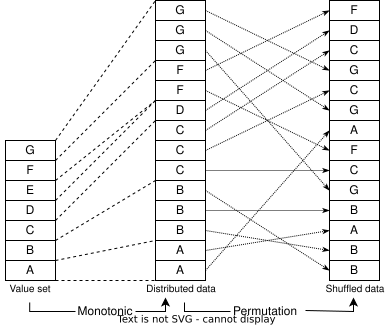
\includegraphics[height=0.5\textwidth]{diagram/distribution}
    
    Kétfázisú értékkiosztás alapelve: \par
    visszafejthető disztribúció és permutáció kompozíciója
\end{frame}

\begin{frame}
    \slidetitle{\sectionshorttitle}{Az értékkészlet interfész-tulajdonságai}
    
    \begin{itemize}
        \setlength\itemsep{1em}
        \item Rendezett \pause
        \item Nincs ismétlődés (unique) \pause
        \item Lekérhető a lista hossza \pause
        \item Lekérhető az adott pozíción lévő érték (random access) \pause
        \item Lekérhető az adott érték pozíciója (reverse index) \pause \par
              ~ ~ ~ (ha az érték nem található, akkor a rendezés szerinti helye) \pause
        \item A lekérések gyorsan hajtódnak végre
    \end{itemize}
\end{frame}

\begin{frame}
    \slidetitle{\sectionshorttitle}{Tipikus értékkészletek}
    
    \begin{itemize}
        \setlength\itemsep{1em}
        \item Szavak/kifejezések előre adott, rendezett listája \pause
        \item Numerikus sáv (például számok 1-től $n$-ig) \pause
        \item Reguláris kifejezésre illeszkedő szövegek \pause
        \item 
    \end{itemize}
\end{frame}

\begin{frame}
    \slidetitle{\sectionshorttitle}{Monotonic implementációk}

    Monotonic...
\end{frame}

\begin{frame}
    \slidetitle{\sectionshorttitle}{Permutation implementációk}

    Permutation...
\end{frame}

\begin{frame}
    \slidetitle{\sectionshorttitle}{Kétfázisú értékkiosztás: adatlekérés}
    
    \centering
    
    \begin{overprint}
        \onslide<1>\centerline{\includegraphics[height=0.45\textwidth]{diagram/getvalue-0}}
        \onslide<2>\centerline{\includegraphics[height=0.45\textwidth]{diagram/getvalue-1}}
        \onslide<3>\centerline{\includegraphics[height=0.45\textwidth]{diagram/getvalue-2}}
        \onslide<4>\centerline{\includegraphics[height=0.45\textwidth]{diagram/getvalue-3}}
        \onslide<5>\centerline{\includegraphics[height=0.45\textwidth]{diagram/getvalue-4}}
        \onslide<6->\centerline{\includegraphics[height=0.45\textwidth]{diagram/getvalue-5}}
    \end{overprint}
    
    \hspace{0.7cm}
    
    Adatlekérés a kétfázisú értékkiosztásból
\end{frame}

\begin{frame}
    \slidetitle{\sectionshorttitle}{Kétfázisú értékkiosztás: keresés}
    
    \centering
    
    \begin{overprint}
        \onslide<1>\centerline{\includegraphics[height=0.45\textwidth]{diagram/findvalue-0}}
        \onslide<2>\centerline{\includegraphics[height=0.45\textwidth]{diagram/findvalue-1}}
        \onslide<3>\centerline{\includegraphics[height=0.45\textwidth]{diagram/findvalue-2}}
        \onslide<4->\centerline{\includegraphics[height=0.45\textwidth]{diagram/findvalue-3}}
    \end{overprint}
    
    \vspace{0.5cm}
    
    Keresés a kétfázisú értékkiosztásban: \par
    A megfordíthatóság biztosítja a hatékony keresést
\end{frame}

\begin{frame}
    \slidetitle{\sectionshorttitle}{Kétfázisú értékkiosztás: nincs találat}
    
    \centering
    
    \begin{overprint}
        \onslide<1>\centerline{\includegraphics[height=0.45\textwidth]{diagram/findvalue-0}}
        \onslide<2>\centerline{\includegraphics[height=0.45\textwidth]{diagram/findvalue2-1}}
        \onslide<3>\centerline{\includegraphics[height=0.45\textwidth]{diagram/findvalue2-2}}
    \end{overprint}
    
    \vspace{0.5cm}
    
    Keresés a kétfázisú értékkiosztásban: \par
    A megfordíthatóság biztosítja a hatékony keresést
\end{frame}

\begin{frame}
    \slidetitle{\sectionshorttitle}{Kétfázisú értékkiosztás: nincs ilyen érték}
    
    \centering
    
    \begin{overprint}
        \onslide<1>\centerline{\includegraphics[height=0.45\textwidth]{diagram/findvalue-0}}
        \onslide<2>\centerline{\includegraphics[height=0.45\textwidth]{diagram/findvaluenone-1}}
        \onslide<3>\centerline{\includegraphics[height=0.45\textwidth]{diagram/findvaluenone-2}}
    \end{overprint}
    
    \vspace{0.5cm}
    
    Keresés a kétfázisú értékkiosztásban: \par
    A megfordíthatóság biztosítja a hatékony keresést
\end{frame}

\begin{frame}
    \slidetitle{\sectionshorttitle}{Kétfázisú értékkiosztás: értéksáv keresése}
    
    \centering
    
    \includegraphics[height=0.45\textwidth]{diagram/findvaluerange}
    
    \vspace{0.5cm}
    
    Keresés a kétfázisú értékkiosztásban: \par
    A megfordíthatóság biztosítja a hatékony keresést
\end{frame}

\section{Konfiguráció és bővítés}
\def\sectionshorttitle{Konfiguráció és bővítés}

\begin{frame}
    \slidetitle{\sectionshorttitle}{Elvárások a konfigurációval szemben}
    
    Elvárások a konfigurációval, bővítéssel, tuningolással szemben
\end{frame}

\begin{frame}
    \slidetitle{\sectionshorttitle}{Konfiguráció-példa}
    
    Konfiguráció-példa (JPA-példa is?)
    [szóban: utalás rá, hogy a végén mutatok majd linket a példarepóra]
\end{frame}

\begin{frame}
    \slidetitle{\sectionshorttitle}{Egyedi működés hozzáadása}
    
    Egyedi működés hozzáadása (pl. valuesSource, valuesResource)
\end{frame}

\begin{frame}
    \slidetitle{\sectionshorttitle}{Bővítés: valós címadatbázis}
    
    Bővítés: valós címek használata
\end{frame}

\begin{frame}
    \slidetitle{\sectionshorttitle}{Bővítés: on-demand schema}
    
    Bővítés: on-demand schema
    [szóban: ez annyira általános, hogy valószínűleg általánosan megcsinálom majd]
\end{frame}

\section{Eredmények}
\def\sectionshorttitle{Eredmények}

\begin{frame}
    \slidetitle{\sectionshorttitle}{Tesztelési módszertan}
    
    Bevezetés az eredményekhez
\end{frame}

\begin{frame}
    \slidetitle{\sectionshorttitle}{Tárhelyigény}
    
    Docker, JAR, adatméret
\end{frame}

\begin{frame}
    \slidetitle{\sectionshorttitle}{Integrált teszt futási ideje (Micronaut$,$ REST)}
    
    \centering
    
    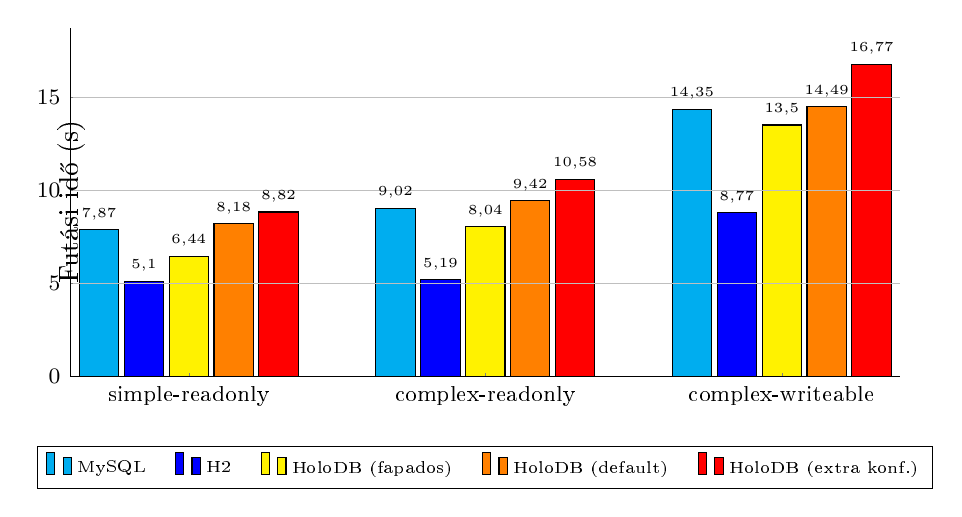
\begin{tikzpicture}[font=\tiny]
        \begin{axis}[
                symbolic x coords={simple-readonly,complex-readonly,complex-writeable},
                ybar,
                axis on top,
                width={\textwidth},
                height=6cm,
                bar width=0.5cm,
                ymajorgrids,
                tick align=inside,
                enlarge y limits={value=.1,upper},
                enlarge x limits=0.2,
                ymin=0,
                ymax=17,
                /pgf/number format/.cd,
                use comma,
                1000 sep={~},
                axis x line*=bottom,
                axis y line*=left,
                tickwidth=1pt,
                legend style={
                    at={(0.5,-0.2)},
                    anchor=north,
                    legend columns=-1,
                    font = {\fontsize{6 pt}{10 pt}\selectfont},
                    /tikz/every even column/.append style={column sep=0.3cm}
                },
                ylabel={Futási idő (s)},
                y label style={at={(0.03,0.5)}},
                xtick=data,
                nodes near coords={
                    \pgfmathprintnumber{\pgfplotspointmeta}
                }
            ]
            \addplot[fill=cyan] % MySQL
                coordinates {
                    (simple-readonly,7.870093628)
                    (complex-readonly,9.0179515675)
                    (complex-writeable,14.3489598653)
                };
            \addplot[fill=blue] % H2
                coordinates {
                    (simple-readonly,5.103988787)
                    (complex-readonly,5.1902669386)
                    (complex-writeable,8.7714582641)
                };
            \addplot[fill=yellow] % HoloDB (fapados)
                coordinates {
                    (simple-readonly,6.441775179)
                    (complex-readonly,8.0399578991)
                    (complex-writeable,13.4957423082)
                };
            \addplot[fill=orange] % HoloDB (default)
                coordinates {
                    (simple-readonly,8.182373242)
                    (complex-readonly,9.4207860077)
                    (complex-writeable,14.4941282014)
                };
            \addplot[fill=red] % HoloDB (extra konf.)
                coordinates {
                    (simple-readonly,8.819935654)
                    (complex-readonly,10.5782986771)
                    (complex-writeable,16.7720866313)
                };
            \legend{MySQL,H2,HoloDB (fapados),HoloDB (default),HoloDB (extra konf.)}
        \end{axis}
    \end{tikzpicture}
\end{frame}

\begin{frame}
    \slidetitle{\sectionshorttitle}{Átlagos futási idők összehasonlítása (log.)}
    
    \centering
    
    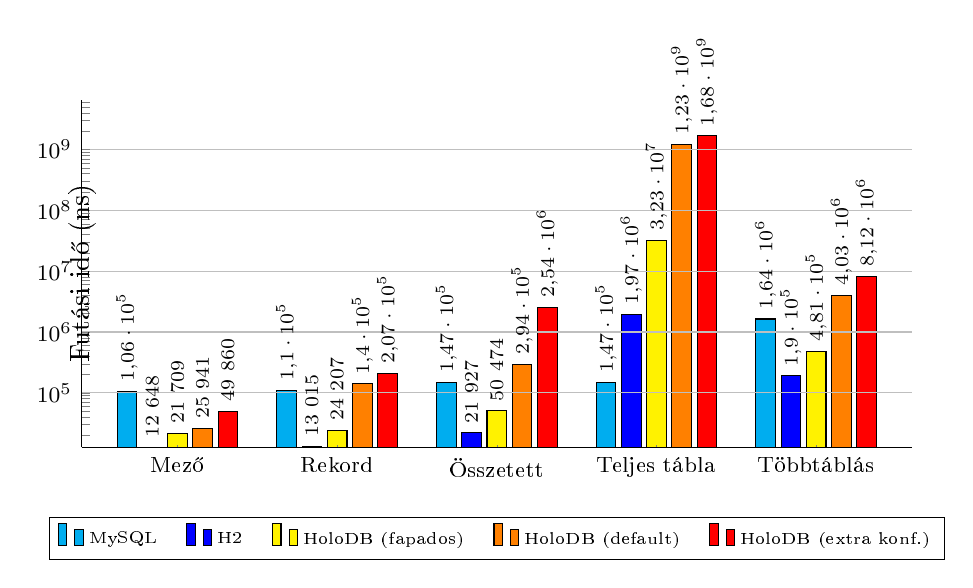
\begin{tikzpicture}[font=\scriptsize]
        \begin{axis}[
                title style={
                    at={(-0.1,1.15)},
                    anchor=north west
                },
                symbolic x coords={Mező,Rekord,Összetett,Teljes tábla,Többtáblás},
                ybar,
                axis on top,
                width={\textwidth},
                height=6cm,
                bar width=0.25cm,
                ymajorgrids,
                tick align=inside,
                enlarge y limits={value=.1,upper},
                enlarge x limits=0.15,
                ymin=0,
                ymax=2000000000,
                ymode=log,
                point meta=rawy,
                /pgf/number format/.cd,
                use comma,
                1000 sep={~},
                every node near coord/.append style={
                    anchor=west,
                    rotate=90
                },
                axis x line*=bottom,
                axis y line*=left,
                tickwidth=1pt,
                legend style={
                    at={(0.5,-0.2)},
                    anchor=north,
                    legend columns=-1,
                    font = {\fontsize{6 pt}{10 pt}\selectfont},
                    /tikz/every even column/.append style={column sep=0.3cm}
                },
                ylabel={Futási idő (ns)},
                y label style={at={(0.03,0.5)}},
                xtick=data,
                nodes near coords={
                    \pgfmathprintnumber{\pgfplotspointmeta}
                }
            ]
            \addplot[fill=cyan] % MySQL
                coordinates {
                    (Mező,106276)
                    (Rekord,109819) 
                    (Összetett,146710)
                    (Teljes tábla,146710)
                    (Többtáblás,1637889)
                };
            \addplot[fill=blue] % H2
                coordinates {
                    (Mező,12648)
                    (Rekord,13015) 
                    (Összetett,21927)
                    (Teljes tábla,1971234)
                    (Többtáblás,189958)
                };
            \addplot[fill=yellow] % HoloDB (fapados)
                coordinates {
                    (Mező,21709)
                    (Rekord,24207) 
                    (Összetett,50474)
                    (Teljes tábla,32271101)
                    (Többtáblás,481306)
                };
            \addplot[fill=orange] % HoloDB (default)
                coordinates {
                    (Mező,25941)
                    (Rekord,140232) 
                    (Összetett,293885)
                    (Teljes tábla,1228183178)
                    (Többtáblás,4030303)
                };
            \addplot[fill=red] % HoloDB (extra konf.
                coordinates {
                    (Mező,49860)
                    (Rekord,207383) 
                    (Összetett,2543441)
                    (Teljes tábla,1676796378)
                    (Többtáblás,8121736)
                };
            \legend{MySQL,H2,HoloDB (fapados),HoloDB (default),HoloDB (extra konf.)}
        \end{axis}
    \end{tikzpicture}
\end{frame}

\section{Összegzés}
\def\sectionshorttitle{Összegzés}

\begin{frame}
    \slidetitle{\sectionshorttitle}{Elvárások teljesítése}
    
    \begin{itemize}
        \setlength\itemsep{0.5em}
        \item[] \onslide<2->{\greencheck} relációs adatmodellre épül
        \item[] \onslide<3->{\greencheck} deklaratív, finomhangolható, könnyen bővíthető
        \item[] \onslide<4->{\greencheck} nem szükséges forrásadatbázis, de mintaként használható
        \item[] \onslide<5->{\greencheck} nincs preparálási folyamat, szinte azonnal elindul
        \item[] \onslide<6->{\greencheck} óriás adatmennyiséget is képes szimulálni, szinte tárhelyigény nélkül
        \item[] \onslide<7->{\greencheck} az adatokat csak elérésükkor, on-the-fly számítja
        \item[] \onslide<8->{\greencheck} a runtime teljesítmény kielégítő
        \item[] \onslide<9->{\greencheck} determinisztikus, konzisztens, skálázható
        \item[] \onslide<10->{\greencheck} opcionálisan írható
    \end{itemize}
\end{frame}

\begin{frame}
    \slidetitle{\sectionshorttitle}{További előnyök}
    
    TODO
\end{frame}

\begin{frame}
    \slidetitle{\sectionshorttitle}{?????}
    
    TODO
\end{frame}

\begin{frame}
    \slidetitle{\sectionshorttitle}{Miért nem terjedt még el hasonló megoldás?}

    \begin{itemize}
        \setlength\itemsep{1em}
        \pause \item \textbf{kontraintuitivitás}:
            előzetes feltevésemmel szemben úgy tűnik, nem olyan egyszerű átlátni a koncepciót,
            és megérteni hogy ``hol is vannak az adatok''
        \pause \item \textbf{megfelelő SQL plannerek eddigi hiánya}:
            az Apache Calcite például csak az utóbbi néhány évben vált népszerűvé,
            és inkább elsősorban adatintegrátorként
        \pause \item \textbf{bejáratott alternatívák}:
            az on-the-fly mockolás lehetősége,
            a NoSQL adatbázisok és felhőmegoldások fejlődése stb.
            sztenderdképző kerülőmegoldásokként elfedték a problémát
        \pause \item \textbf{érdekhiány}:
            nincs nyomás jelentősen más típusú termékkel való kísérletezésre,
            a nagy adatbázisvendorok érdeke elsősorban
            a tényleges adatbázisok kezelésére kínált megoldások fejlesztése
    \end{itemize}
\end{frame}

\begin{frame}
    \slidetitle{\sectionshorttitle}{Jövőbeli tervek}

    \begin{itemize}
        \setlength\itemsep{1em}
        
        \item TODO
    \end{itemize}
\end{frame}
        
\begin{frame}
    \vspace{1em}
    
    \centering
    
    { \Huge Köszönöm a figyelmet! }
    
    \vspace{3em}
    
    \begin{flushleft}
        \normalsize
        
        ~~~
        { \color{beamer@blendedblue} Projektlinkek: }
        
        \vspace{0.5em}
        
        \footnotesize
        
        \begin{itemize}
            \item HoloDB projekt: \par
                    \url{https://github.com/miniconnect/holodb}
            \item Használati példák: \par
                    \url{https://github.com/miniconnect/general-docs/tree/main/examples}
            \item Jelen TDK-pályamunka forrásrepója: \par
                    \url{https://github.com/davidsusu/holodb-tdk}
        \end{itemize}
    
        \vspace{1.5em}
        
        \normalsize
        
        ~~~
        { \color{beamer@blendedblue} E-mail: }
        \href{mailto:horvathdown@student.elte.hu}{horvathdown@student.elte.hu}
        \end{flushleft}
\end{frame}

\end{document}
